% Pengaturan ukuran teks dan jenis dokumen
\documentclass[11pt]{article}

% Pengaturan ukuran halaman dan margin
\usepackage[a4paper,top=30mm,left=30mm,right=20mm,bottom=20mm]{geometry}

% Pengaturan ukuran spasi
\usepackage[singlespacing]{setspace}

% Judul dokumen
\title{Proposal Pra Tugas Akhir ITS}
\author{Rifqi Alhakim Hariyantoputera}

% Pengaturan format bahasa
\usepackage[indonesian]{babel}

% Pengaturan detail pada file PDF
\usepackage[pdfauthor={\@author},bookmarksnumbered,pdfborder={0 0 0}]{hyperref}

% Pengaturan jenis karakter
\usepackage[utf8]{inputenc}

% Pengaturan ukuran indentasi
\setlength{\parindent}{2em}

% Package lainnya
\usepackage{etoolbox} % Mengubah fungsi default
\usepackage{enumitem} % Pembuatan list
\usepackage{lipsum} % Pembuatan template kalimat
\usepackage{graphicx} % Input gambar
\usepackage{longtable} % Pembuatan tabel
\usepackage[table,xcdraw]{xcolor} % Pewarnaan tabel
\usepackage[numbers]{natbib} % Kutipan artikel
\usepackage{changepage} % Pembuatan teks kolom
\usepackage{multicol} % Pembuatan kolom ganda
\usepackage{multirow} % Pembuatan baris ganda
\usepackage{float}
\usepackage{outlines}

% Pengaturan format judul bab
\usepackage{titlesec}
\renewcommand{\thesection}{\arabic{section}}
\titleformat*{\section}{\normalsize\bfseries}
\titlespacing{\section}{0ex}{3ex}{1.5ex}
\titleformat*{\subsection}{\normalsize\bfseries}
\titlespacing{\subsection}{0ex}{3ex}{1.5ex}
\titleformat*{\subsubsection}{\normalsize\bfseries}
\titlespacing{\subsubsection}{5ex}{1ex}{1ex}
% \titleformat*{\subsection}{\normalsize\bfseries}
% \titlespacing{\subsection}{0ex}{3ex}{1.5ex}

% Isi keseluruhan dokumen
\begin{document}

  % Menonaktifkan penomoran halaman
  \pagenumbering{gobble}

  % Lembar pengesahan
  \begin{flushleft}
    % Ubah kalimat berikut sesuai dengan nama departemen dan fakultas
    \textbf{Departemen Teknik Komputer - FTEIC}\\
    \textbf{Institut Teknologi Sepuluh Nopember}\\
  \end{flushleft}
  
  \begin{center}
    % Ubah detail mata kuliah berikut sesuai dengan yang ditentukan oleh departemen
    \underline{\textbf{EC184701 - PRA TUGAS AKHIR (2 SKS)}}
  \end{center}
  
  \begin{adjustwidth}{-0.2cm}{}
    \begin{tabular}{lcp{0.7\linewidth}}
  
      % Ubah kalimat-kalimat berikut sesuai dengan nama dan NRP mahasiswa
      Nama Mahasiswa &:& Rifqi Alhakim Hariyantoputera \\
      NRP &:& 07211840000055 \\
  
      % Ubah kalimat berikut sesuai dengan semester pengajuan proposal
      Semester &:& Ganjil 2021/2022 \\
  
      % Ubah kalimat-kalimat berikut sesuai dengan nama-nama dosen pembimbing
      Dosen Pembimbing &:& 1. Dr. Eko Mulyanto Yuniarno, S.T., M.T. \\
      & & 2. Reza Fuad Rachmadi, S.T., M.T., Ph.D. \\
  
      % Ubah kalimat berikut sesuai dengan judul tugas akhir
      Judul Tugas Akhir &:& \textbf{Smart Whiteboard: Pengenalan Teks Huruf Balok } \\
      & & \textbf{Menggunakan You Only Look Once (YOLO)} \\
  
      Uraian Tugas Akhir &:& \\
    \end{tabular}
  \end{adjustwidth}
  
  % Ubah paragraf berikut sesuai dengan uraian dari tugas akhir
  Tulisan merupakan salah satu bentuk ragam komunikasi. Dengan adanya tulisan, suatu ide atau gagasan dapat dituangkan dan dan diabadikan. Segmentasi dokumen gambar menjadi suatu bentuk kalimat merupakan Langkah penting untuk memahami suatu dokumen secara utuh. Walaupun diklaim memiliki akurasi hingga 99\%, Optical Character Recognition (OCR) yang ada saat ini memiliki penurunan akurasi ketika dihadapkan kepada gambar dengan kualitas rendah. Berbagai teknologi Internet of Things diterapkan pada papan tulis sehingga memiliki fitur tambahan yang dapat mempermudah proses belajar dan mengajar. Telah banyak teknologi yang dapat memproyeksikan gambar atau tulisan pada computer ke papan tulis pintar. Namun, belum ada teknologi yang mampu mengenali tulisan tangan pada papan tulis pintar. Maka dari itu, diperlukannya suatu algoritma atau program untuk mendeteksi dan klasifikasi teks huruf balok untuk diterapkan pada alat Smart Whiteboard. Sehingga didapatkan tujuan akhir yaitu untuk membuat program komputer yang dapat melakukan pengenalan teks huruf balok menggunakan YOLO sehingga dapat diimplementasikan pada alat Smart Whiteboard.
    
  \vspace{1ex}
  
  \begin{flushright}
    % Ubah kalimat berikut sesuai dengan tempat, bulan, dan tahun penulisan
    Surabaya, Desember 2021
  \end{flushright}
  \vspace{1ex}
  
  \begin{center}
  
    \begin{multicols}{2}
  
      Dosen Pembimbing 1
      \vspace{12ex}
  
      % Ubah kalimat-kalimat berikut sesuai dengan nama dan NIP dosen pembimbing pertama
      \underline{[Dr. Eko Mulyanto Yuniarno, S.T., M.T.]} \\
      NIP. 196806011995121000
  
      \columnbreak
  
      Dosen Pembimbing 2
      \vspace{12ex}
  
      % Ubah kalimat-kalimat berikut sesuai dengan nama dan NIP dosen pembimbing kedua
      \underline{[Reza Fuad Rachmadi, S.T., M.T., Ph.D.]} \\
      NIP. 198504032012121000
  
    \end{multicols}
    \vspace{6ex}
  
    Mengetahui, \\
    % Ubah kalimat berikut sesuai dengan jabatan kepala departemen
    Kepala Departemen Teknik Komputer FTEIC - ITS
    \vspace{12ex}
  
    % Ubah kalimat-kalimat berikut sesuai dengan nama dan NIP kepala departemen
    \underline{Dr. Supeno Mardi Susiki Nugroho, S.T., M.T.} \\
    NIP. 197003131995121001
  
  \end{center}
  \newpage

  \begin{center}
    % Ubah judul
    \textbf{Smart Whiteboard: Pengenalan Teks Huruf Balok Menggunakan You Only Look Once (YOLO)}
  \end{center}

  % Konten pendahuluan
  \section{PENDAHULUAN}

\subsection{Latar Belakang}

% Ubah paragraf-paragraf berikut sesuai dengan latar belakang dari tugas akhir
Komunikasi, pada dasarnya merupakan aktivitas dasar manusia. Dengan adanya komunikasi, manusia dapat saling berhubungan dengan satu sama lain. Tulisan merupakan salah satu bentuk ragam komunikasi. Dengan adanya tulisan, suatu ide atau gagasan dapat dituangkan dan disampaikan kepada pembaca secara asinkronus serta dapat diabadikan. Secara umum, ragam tulisan dibagi menjadi 2 yaitu tulisan cetak pada dokumen dan tulisan tangan.\par
Segmentasi dokumen gambar menjadi suatu bentuk kalimat merupakan Langkah penting untuk memahami suatu dokumen. Tidak seperti dokumen cetak, segmentasi pada dokumen bertulisan tangan masih merupakan suatu hal yang menantang karena memiliki ukuran spacing yang tidak menentu antar hurufnya serta memiliki variasi bentuk gaya tulisan \citep*{ryu2015word}. Tulisan cetak pada dokumen merupakan tulisan yang pengaturan dan gaya penulisannya diatur dan dikenali oleh program computer.\par
\textit{Optical Character Recognition (OCR)} adalah proses konversi gambar huruf menjadi karakter ASCII yang dikenali oleh komputer. Walaupun diklaim memiliki akurasi hingga 99\%, \textit{Optical Character Recognition (OCR)} yang ada saat ini memiliki penurunan akurasi ketika dihadapkan kepada gambar dengan kualitas rendah seperti \textit{noise} gambar, kualitas cetakan rendah, karakter berdekatan \citep*{ImageMalu2001approachtch}, dan karakter dengan variasi yang tidak umum (tulisan tangan).\par
Papan tulis merupakan suatu media yang biasa digunakan untuk menuangkan tulisan, ide, ataupun gagasan dalam proses belajar dan mengajar. Seiring dengan perkembangan teknologi, berbagai teknologi \textit{Internet of Things} diterapkan pada papan tulis sehingga memiliki fitur tambahan yang dapat mempermudah proses belajar dan mengajar. Telah banyak teknologi yang dapat memproyeksikan gambar atau tulisan pada computer ke papan tulis pintar \citep*{kellerman2018smart}. Namun, belum ada teknologi yang mampu mengenali tulisan tangan pada papan tulis pintar.



\subsection{Permasalahan}

% Ubah paragraf berikut sesuai dengan permasalahan dari tugas akhir
Permasalahan yang didapat yaitu diperlukannya suatu metode untuk mendeteksi dan klasifikasi teks huruf balok untuk diterapkan pada alat \textit{Smart Whiteboard.} 

\subsection{Penelitian Terkait}
% Ubah paragraf berikut sesuai dengan penelitian lain yang terkait dengan tugas akhir

\subsubsection{Penelitian Berkaitan dengan \textit{Smart Whiteboard}}
Kellerman et al. \citep*{kellerman2018smart} mencoba untuk menyediakan suatu cara alternatif dan terjangkau pada papan tulis atau slides agar bisa mendapat interaksi lebih dari murid serta untuk meningkatkan efisiensi dari pengajaran. Pada penelitiannya, peneliti membuat sebuah papan tulis interaktif menggunakan Nintendo Wii \textit{Remote} dan \textit{PC Suite}. \textit{Software Suite} yang dikembangkan memungkinkan tampilan PC apapun dapat digunakan sebagai papan tulis interaktif. Sistem yang dibangun memiliki fungsi yang diperlukan untuk menciptakan sarana pembelajaran yang lebih baik dan lebih berteknologi, serta memberi pengguna dan siswa alat tambahan untuk menunjang Pendidikan interaktif. \textit{PC Suite} dibuat seramah mungkin sehingga dapat digunakan dengan mudah pada komputer standar.\

\subsubsection{Penelitian Berkaitan dengan \textit{Word Detection}}
Arun et al. \citep*{arun2019handwritten} menyajikan pendekatan sederhana untuk segmentasi huruf kata tulisan tangan menggunakan pendekatan bounding box dan pendekatan berbasis pixel. Segmentasi huruf tulisan tangan merupakan proses yang menantang karena gaya penulisan yang bervariasi. Kata-kata tulisan tangan yang tidak bersentuhan disegmentasikan dengan pendekatan bounding box dan kata-kata tulisan tangan yang bersentuhan disegmentasi menggunakan pendekatan pixel. Paper ini mencapai tingkat segmentasi hingga 94.45\% dan tingkat pengenalan 85.89\% dengan skema training dan testing 50-50\%.

\subsubsection{Penelitian Berkaitan dengan YOLO \textit{Object Detection}}
Karlina dan Indarti \citep*{karlina2020pengenalan} membuat pengenalan objek karlina2020pengenalan cepat saji dari \textit{video} dan \textit{real time webcam} menggunakan metode \textit{deep learning. You Only Look Once (YOLO)} merupakan model \textit{deep learning} yang digunakan untuk pengenalan objek. Jumlah data yang digunakan terdiri dari 468 gambar yang terdiri dari 3 jenis karlina2020pengenalan cepat saji. Nilai avg loss pada model akhir yang dibangun yaitu 4.6\%, nilai validasi mAP 100\%, serta akurasi akhir berkisar antara 63\% sampai 100\%.

\subsection{Gap Penelitian}
Pada penelitian berkaitan dengan \textit{smart whiteboard} \citep*{kellerman2018smart} telah dibuat \textit{smart whiteboard} yang dapat mendeteksi huruf yang dibuat dengan alat, namun tidak dapat mendeteksi tulisan yang dibuat pada papan tulis. Kemudian, pada penelitian berkaitan dengan \textit{word detection} \citep*{ryu2015word} \citep*{arun2019handwritten} telah dibuat algoritma pendeteksi huruf menggunakan pendekatan textit{structure learning, bounding box,} dan \textit{pixel based,} namun tidak menggunakan metode \textit{You Only Look Once (YOLO).} Sedangkan pada penelitian berkaitan dengan \textit{YOLO Object Detection} \citep*{karlina2020pengenalan} YOLO digunakan untuk deteksi objek berupa karlina2020pengenalan cepat saji, namun tidak digunakan untuk deteksi huruf balok pada papan tulis pintar.

\subsection{Tujuan Penelitian}
Tujuan dari dibuatnya tugas akhir ini yaitu untuk membuat program komputer yang dapat melakukan pengenalan teks huruf balok sehingga dapat diimplementasikan pada alat \textit{Smart Whiteboard.}

  % Konten tinjauan pustaka
  \section{TINJAUAN PUSTAKA}

\subsection{\textit{Convolutional  Neural Network (CNN)}}
CNN merupakan algoritma \textit{deep learning} yang mampu mengambil masukan berupa gambar, menetapkan prioritas untuk berbagai aspek/objek dalam gambar dan mampu membedakan satu sama lain. Tahapan \textit{pre-processing} yang dibutuhkan CNN lebih sedikit jika dibandingkan dengan algoritma klasifikasi lainnya \citep*{towardsDS}.

% Contoh penggunaan referensi dari pustaka
% Newton pernah merumuskan \citep{Newton1687} bahwa \lipsum[8]
% Contoh penggunaan referensi dari persamaan
% Kemudian menjadi persamaan seperti pada persamaan \ref{eq:FirstLaw}.

\subsection{\textit{You Only Look Once (YOLO)}}
YOLO merupakan salah satu arsitektur dari CNN yang dioptimasi untuk mendeteksi objek pada gambar. Arsitektur YOLO sangat cepat apabila dibandingkan dengan arsitektur pengenalan objek lainnya \citep*{jeong2018image}. 

% % input gambar
% \begin{figure} [H] \centering
%     % Nama dari file gambar yang diinputkan
%     \includegraphics[scale=0.6]{gambar/umur.png}
%     % Keterangan gambar yang diinputkan
%     \caption{Kategori umur menurut Depkes. RI (2009)}
%     % Label referensi dari gambar yang diinputkan
%     \label{fig:Umur}
% \end{figure}

\subsection{\textit{Word Segmentation}}
Pengenalan tulisan tangan merupakan Teknik untuk menginterpretasikan tulisan tangan kedalam bentuk digital. Proses pengenalan tulisan tangan dapat diperoleh dengan 2 cara yaitu dengan mengonversi otomatis karakter pada saat ditulis pada layar sentuh dengan pena digital dan cara lain yaitu dengan melakukan pengambilan gambar serta pemrosesan gambar pada suatu teks yang ingin dikenali [8]. Pada proses segmentasi huruf, mulanya dokumen gambar disegmentasi kedalam baris-baris teks. Kemudian, algoritma segmentasi huruf diterapkan pada satu baris teks tersebut. Pada satu baris teks tersebut, secara umum proses segmentasi huruf konvensional menjalankan algoritma yang terdiri dari 2 tahapan yaitu: ekstraksi kandidat huruf berdasarkan pemisah huruf dan dilanjut dengan klasifikasi kandidat huruf \citep*{ryu2015word}.

% \subsection{Deep Learning}
%  Deep Learning merupakan artificial neural network yang memiliki banyak layer dan synapse weight. 
%  Deep learning dapat menemukan relasi tersembunyi atau pola yang rumit antara input dan output, yang 
%  tidak dapat diselesaikan menggunakan multilayer perceptron. Keuntungan  utama  deep  learning  yaitu 
%  mampu merubah data dari nolinearly separable menjadi linearly separable melalui serangkaian transformasi 
%  (hidden layers). Selain itu, deep learning juga mampu mencari decision boundary yang berbentuk non-linier
%  , serta mengsimulasikan interaksi non-linier antar fitur. Jadi, input ditransformasikan secara 
%  non-linier sampai akhirnya pada output, berbentuk distribusi class-assignment\citep{DeepLearning}.

%  \begin{figure} [H] \centering
%     % Nama dari file gambar yang diinputkan
%     \includegraphics[scale=0.6]{gambar/deeplearning.png}
%     % Keterangan gambar yang diinputkan
%     \caption{Deep Learning 4 layer}
%     % Label referensi dari gambar yang diinputkan
%     \label{fig:Deep Learning}
% \end{figure}

% \subsection{Convolutional Neural Network (CNN)}
% Convolutional Neural Network (CNN) merupakan cabang dari Multilayer Perceptron (MLP) yang digunakan untuk
% mengolah data dua dimensi. CNN memiliki kedalaman jaringan yang tinggi sehingga CNN termasuk dalam jenis
% Deep Neural Network. Perbedaan CNN dengan MLP terdapat pada neuron dimana pada MLP setiap neuron hanya
% berukuran satu dimensi, sedangkan CNN setiap neuronnya berukuran dua dimensi. Pada CNN, operasi linier
% menggunakan operasi konvolusi\citep{CNN}.

% \subsection{Image Processing}
% Image Processing atau Pengolahan Citra merupakan teknik dalam pemrosesan gambar dengan input berupa 
% citra dua dimensi yang bertujuan untuk menyempurnakan citra atau mendapatkan informasi yang berguna 
% untuk diolah menjadi beberapa keputusan. Dalam operasi pemrosesan citra, operasi yang sering dilakukan 
% dalam format gambar grayscale. Gambar grayscale didapatkan dari pemrosesan gambar berwarna yang 
% didekomposisi menjadi komponen merah (R), hijau (G) dan biru (B) yang diproses secara independen sebagai 
% gambar grayscale. Image Processing terbagi menjadi dalam tiga tingkatan\citep{ImageProcesing}:
%     \begin{enumerate}
%         \item Low-Level Image Processing \\
%         Low-Level Image Processing merupakan operasi sederhana dalam pengolahan gambar dimana input dan 
%         output berupa gambar. Contoh: contrast enchancement dan noise reduction.
%         \item Mid-Level Image Processing \\
%         Mid-Level Image Processing merupakan operasi pengolahan gambar yang melibatkan ekstrasi atribut dari 
%         gambar input. Contoh: edges, contours dan regions.
%         \item High-Level Image Processing \\
%         High-Level Image Processing merupakan merupakan kategoriyang melibatkan pemrosesan gambar kompleks 
%         yang terkait dengan analisis dan interpretasi konten dalam sebuah keadaan untuk pengambilan keputusan.
%     \end{enumerate}




  % Konten metodologi
  \section{METODOLOGI}

% Ubah konten-konten berikut sesuai dengan isi dari metodologi

\subsection{Data dan Peralatan}

\subsubsection{Data}
Dataset yang akan digunakan dalam proses pembuatan tugas akhir ini yaitu dataset buatan peneliti. Adapun rencana pembuatan dataset yaitu dataset berdasarkan beberapa tulisan tangan dari rekan peneliti yang ditulis disebuah papan tulis dan kemudian diambil gambarnya dalam beberapa pengaturan sudut, resolusi, serta pencahayaan yang berbeda.

\subsubsection{Peralatan}
\begin{itemize}
   \item [a.] Laptop \\
   Laptop merupakan perangkat keras (Hardware) yang berfungsi untuk mengolah data. Laptop yang digunakan pada penelitian tugas akhir memiliki spesifikasi Intel Core i5-8300H 2.3 GHz (8 CPUs), HDD Storage 1 TB, SSD Storage 256 GB, RAM 16 GB DDR4 2666 MHz, Graphic Card NVIDIA GeForce GTX 1050 Ti 4GB GDDR5.

   \item [b.] Google Colaboratory \\
   Google Colaboratory merupakan sebuah \textit{cloud-based executable code} yang dapat menunjang programmer dalam menjalankan serangkaian kode yang dimilikinya. Keunggulan dari Google Colaboratory yaitu proses eksekusi kode dapat dilakukan secara cloud sehingga dapat meringankan beban kerja pada laptop.
\end{itemize}
   

\subsection{Metodologi Penelitian}
Metodologi yang digunakan dalam pengerjaan Tugas Akhir ini adalah sebagai berikut.
    % Contoh input gambar dengan format *.jpg
    \begin{figure} [H] \centering
      % Nama dari file gambar yang diinputkan
      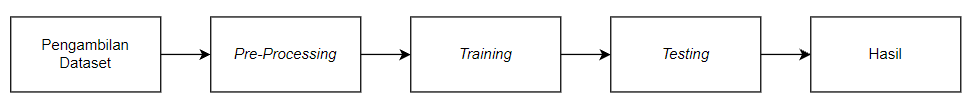
\includegraphics[scale=0.6]{gambar/Metodologi.png}
      % Keterangan gambar yang diinputkan
      \caption{Diagram blok metodologi}
      % Label referensi dari gambar yang diinputkan
      \label{fig:Metodologi}
    \end{figure}

\begin{enumerate}
   \item \textbf{Pengambilan Dataset} \\
   Pada tahapan ini, dilakukan proses pengambilan data berdasarkan kebutuhan pembuatan tugas akhir. Data yang akan dikumpulkan pada tahapan ini yaitu berupa sejumlah foto dari masing-masing huruf balok. Pada tahapan ini pula, dilakukan proses pemberian label pada dataset.
   \item \textbf{Pre-Processing} \\
   Pada tahapan ini, dilakukan \textit{pre-processing} dari dataset yang sebelumnya telah didapat. Pada tahapan ini pula, dataset dibagi menjadi 3 bagian yaitu \textit{data training, data validation dan data testing. }
   \item \textbf{Training} \\
   Pada tahapan ini, dilakukan proses \textit{training} dan \textit{tuning} menggunakan YOLO. Pada proses pembangunan model ini pula ditentukan \textit{epoch, Batch Size, Iteration, dan Loss Function.}
   \item \textbf{Testing} \\
   Pada tahapan ini, dilakukan proses testing yaitu untuk pengujian model yang telah dibangun sebelumnya untuk menentukan apakah model yang telah dibuat dirasa sudah cukup atau perlu dilakukan perubahan konfigurasi kembali dari awal. Pada tahapan ini pula, model dianalisa serta dievaluasi menggunakan \textit{Confusion Matrix.}
   \item \textbf{Hasil} \\
   Pada tahapan ini, jika model telah sesuai dengan threshold dan model telah berfungsi dengan baik, maka proses selanjutnya yaitu pelaporan dalam pembukuan tugas akhir.
\end{enumerate}

  % Konten lainnya
  \section{HASIL YANG DIHARAPKAN}

Hasil yang diharapkan dari tugas akhir ini yaitu terbentuknya program komputer yang dapat melakukan pengenalan teks huruf balok pada papan tulis dan juga dapat diaplikasikan pada alat \textit{Smart Whiteboard.}

\section{RENCANA KERJA}

% Ubah tabel berikut sesuai dengan isi dari rencana kerja
\newcommand{\w}{}
\newcommand{\G}{\cellcolor{gray}}
\begin{table}[h!]
  \begin{tabular}{|p{4cm}|c|c|c|c|c|c|c|c|c|c|c|c|c|c|c|c|}

    \hline
    \multirow{2}{*}{Kegiatan} & \multicolumn{16}{|c|}{Minggu} \\
    \cline{2-17} &
    1 & 2 & 3 & 4 & 5 & 6 & 7 & 8 & 9 & 10 & 11 & 12 & 13 & 14 & 15 & 16 \\
    \hline

    % Gunakan \G untuk mengisi sel dan \w untuk mengosongkan sel
    Pengambilan Dataset &
    \G & \G & \G & \w & \w & \w & \w & \w & \w & \w & \w & \w & \w & \w & \w & \w \\
    \hline

    \textit{Pre-Processing Dataset} &
    \w & \w & \G & \G & \G & \w & \w & \w & \w & \w & \w & \w & \w & \w & \w & \w \\
    \hline

    \textit{Training Model} &
    \w & \w & \w & \w & \G & \G & \G & \G & \G & \w & \w & \w & \w & \w & \w & \w \\
    \hline

    \textit{Testing Model} &
    \w & \w & \w & \w & \w & \w & \G & \G & \G & \G & \G & \w & \w & \w & \w & \w \\
    \hline
    
    Hasil Model &
    \w & \w & \w & \w & \w & \w & \w & \w & \G & \G & \G & \G & \G & \G & \w & \w \\
    \hline

    Dokumentasi dan Pembuatan Laporan &
    \G & \G & \G & \G & \G & \G & \G & \G & \G & \G & \G & \G & \G & \G & \G & \G \\
    \hline

  \end{tabular}
\end{table}

  % Daftar pustaka
  \renewcommand\bibname{DAFTAR PUSTAKA}
  \addcontentsline{toc}{chapter}{\bibname}
  \bibliographystyle{unsrtnat}
  \bibliography{dafpus/pustaka.bib}
  \cleardoublepage
  %\section{DAFTAR PUSTAKA}
  %\renewcommand\refname{}
  %\vspace{-2ex}
  %\bibliographystyle{unsrtnat}
  %\bibliography{pustaka/pustaka.bib}

\end{document}